\documentclass[a4paper]{article}
\usepackage{amsmath}
\usepackage{graphicx}
\usepackage{geometry}
\usepackage{floatrow}
\usepackage{layout}
\usepackage{amssymb} 
\usepackage{multirow}
\usepackage{caption}
\geometry{margin=1in}
\usepackage{authblk}
\usepackage{indentfirst}
\usepackage[hidelinks]{hyperref}
\usepackage{enumitem}
\usepackage{float}
\usepackage{hyperref}
\usepackage{amssymb}
\usepackage{xcolor}
\usepackage{titlesec}

% Define link color
\hypersetup{
    colorlinks=true,
    linkcolor=teal,  % Color for internal links
    filecolor=teal,  % Color for file links
    urlcolor=teal,   % Color for URLs
    citecolor=black  % Color for citation links
}

% Define custom dark teal color
\definecolor{darkteal}{RGB}{0, 102, 102} % Adjust the RGB values as needed

%custom crimson color
\definecolor{crimson}{rgb}{0.86, 0.08, 0.24}

% Define section color
\titleformat{\section}
  {\color{darkteal}\normalfont\Large\bfseries} % Formatting for section titles
  {\thesection}{1em}{}

\providecommand{\keywords}[1]
{
  \small	
  \textbf{\; \textit{Keywords---}} #1
}

\begin{document}

\title{\textbf{\huge{Problem Set + Programming Assignment 3}}}

\author{\textbf\large{Teera Tesharojanasup}}

\affil{\textbf{Northeastern University, Boston}}

\date{\text{August 6th, 2024}}

\maketitle
\begin{sloppypar}

\section*{Overview}

Problem set 3 and Programming Assignment 3 are combined for CS 4100 Summer II. Taught by assistant teaching professor, \href{https://rajagopalvenkat.com/}{Rajagopal Venkat}. \cite{MISC:1}

\section{Loss, Gradients, and PyTorch}

\par \textbf{Preliminaries:} Recall our discussion of loss functions from class. For a multi-class classification problem, given a prediction model $f$, 
a common loss function is the Categorical Cross Entropy loss, which is calculated as follows:

\[ L(x_i, y_i) = -y_i \cdot log(f(x_i))\]

Here, $y_i$ is a one-hot vector (i.e. a vector of length $m$, where $m$ is the number of classes)
with an entry of $1$ in the position corresponding to the true class and $0$ elsewhere. Similarly, 
the model output $f(x_i)$ is a vector, containing the probabilities that the input belongs
to each of the classes.


\begin{enumerate}[start=1,label=Q\arabic*,left=0pt]
    \item \textbf{Consider a logistic regression ($\hat{y}_i = \sigma(w \cdot x_i + b)$) with two classes ($0$ and $1$). Given
    the input example, $x_i = [6, 4, 2, 3, 1]$, model weights $w = [0.5, 0.1, -0.8, 0.9, 0.0]$, bias term,
    $b = 0.05$ and the true label encoded as $y_i = [0, 1]$, compute the cross entropy loss and
    show every step of your calculation. (Hint: a logistic regression gives you the probability of the '1' class.). \hfill \textcolor{teal}{(4)}}
    
    \par
    
    \item \textbf{The Rectified Linear Unit (ReLU) activation function is defined as:}
    
    \[
    ReLU(x) = \frac{x + |x|}{2} = \begin{cases} 
    x & \text{if } x > 0 \\
    0 & \text{otherwise}
    \end{cases}
    \]

    \textbf{Now consider the neural network in the figure below, with 3 possible classes instead.
    Assume that the hidden layer uses the ReLU activation function instead of the sigmoid
    function discussed in class. The final layer uses the sigmoid (logistic function) activation
    function, followed by a \href{https://en.wikipedia.org/wiki/Softmax_function}{Softmax} operation to 
    ensure that the outputs add up to $1$.}

    \begin{figure}[H]
        \centering  
        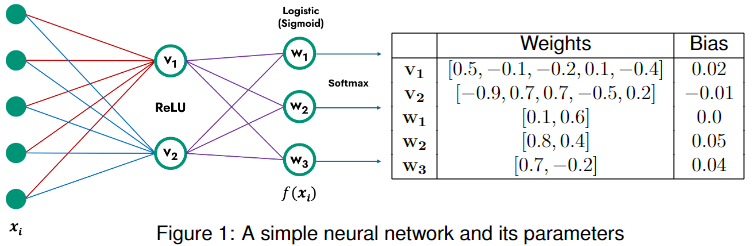
\includegraphics[height=0.18\textheight]{Q2_NN.png}
        \label{fig:Q2_NN}
    \end{figure}

    \textbf{For $x_i = [5, 7, 4, 3, 2]$, and the true class label $2$ (where the possible classes are $0$, $1$, and
    $2$), use the model from the diagram, and the given weights table (including nonzero biases
    this time) to compute the cross entropy loss. You may use NumPy/SciPy operations (but
    not the loss function methods from these packages) to perform the calculations for this
    question - if doing so, paste a screenshot of your function(s) and the final result into your
    written submission. You may find the SciPy expit function useful: \href{https://docs.scipy.org/doc/scipy/reference/generated/scipy.special.expit.html\#scipy.special.expit}{[link]}. \hfill \textcolor{teal}{(6)}}
    
    \par
    
    \item \textbf{Using a computation graph (of the kind we discussed in class), compute the gradient
    of the cross entropy loss with respect to the model parameters in the above network. Repeatedly split 
    the loss function by operators like we did in class, and ignore all bias terms.
    You do not need to split vector/matrix operators into elementwise/row-wise operations.
    For this question alone, you may scan a hand-drawn figure. Any writing must be perfectly
    legible. Finally, use NumPy to compute the value of the gradient of the loss function with
    respect to all parameters ($w_1, w_2, w_3, v_1, v_2$) for the given input and true label. Note that
    the $log$ operator refers to the natural logarithm (base $exp$). Report your final values and a
    screenshot of your code. HINT: \href{https://towardsdatascience.com/derivative-of-the-softmax-function-and-the-categorical-cross-entropy-loss-ffceefc081d1}{[Derivative of Softmax]} \hfill \textcolor{teal}{(5 + 5)}}
    
    \par 

\end{enumerate}

\section{Fashion-MNIST Classification}

\par In this section, you will be working with a dataset called Fashion-MNIST. Your task is to
design and train a neural network that classifies each image of the dataset correctly. Data
is downloaded directly from within the script (using PyTorch). The actual architecture of
the neural network is up to you, and convolutional layers are optional.

\vspace{\baselineskip}

\noindent Fashion-MNIST contains grayscale images of 28 x 28 pixels representing images of clothing. 
The dataset has 60000 training images, and 10000 testing images, and each image
comes with an associated label (e.g. t-shirt, coat, bag, etc.). There are 10 classes, just
like the MNIST handwritten digits dataset, so that it may serve as a direct drop-in replacement 
to test neural networks. Read the full details about this dataset \href{https://github.com/zalandoresearch/fashion-mnist}{at the repository}.

\vspace{\baselineskip}

\noindent The starter code for this part of the assignment is called "fashionmnist.py". The skeleton
code serves as a general guide. There are some sections without any guidelines where
you will be expected to research and experiment with various techniques to find a good
approach. You must use PyTorch in this section, which is well-documented online.

\vspace{\baselineskip}

\noindent \textbf{\textcolor{crimson}{Your accuracy on the testing dataset must be greater or equal to \underline{80\%}.}}

\vspace{\baselineskip}

\begin{enumerate}[start=4,label=Q\arabic*,left=0pt]
    \item \textbf{Submit two figures: A figure containing an image that is classified incorrectly by your
    model. Include a clear label in this figure that indicates the predicted class from your
    model and the true class the image belongs to (both human-readable labels, not just the
    class number). The second figure should be a single image classified correctly by your
    model and its corresponding class label. \hfill \textcolor{teal}{(3)}}

    \par

    \item \textbf{Submit a plot showing your training loss over time. \hfill \textcolor{teal}{(2)}}

    \par 

    \item \textbf{Assume both the testing and training datasets have twice as many coat images as
    shirt images, and answer the following questions: \hfill \textcolor{teal}{(6)}}
    \begin{enumerate}
        \item \textbf{Would accuracy still be a good metric?}
        \item \textbf{How would you modify your accuracy metric to account for data imbalance?}
        \item \textbf{What other metrics can you use to evaluate model performance?}
    \end{enumerate}

    \par 

    \item \textbf{Calculate the total number of tunable parameters your model has. Show your work,
    and don’t forget the bias terms. Do not use code output to answer this question. \hfill \textcolor{teal}{(4)}}

    \par 

\end{enumerate}
\end{sloppypar}

\bibliography{references}
\bibliographystyle{ieeetr}

\end{document}